% !TEX TS-program = xelatex
% !BIB program = bibtex
% !TeX spellcheck = ru_RU

% About magic macros see also
% https://tex.stackexchange.com/questions/78101/

% По умолчанию используется шрифт 14 размера.
% Если Вы не влезаете в лимит страниц и нужен 12-й шрифт,
% то уберите опцию [14pt]
\documentclass[14pt, russian]{matmex-diploma-custom}

% !TeX spellcheck = ru_RU
% !TEX root = vkr.tex
% Опциональные добавления используемых пакетов. Вполне может быть, что они вам не понадобятся, но в шаблоне приведены примеры их использования.
\usepackage{tikz} % Мощный пакет для создание рисунков, однако может очень сильно замедлять компиляцию
\usetikzlibrary{decorations.pathreplacing,calc,shapes,positioning,tikzmark}

% Библиотека для TikZ, которая генерирует отдельные файлы для каждого рисунка
% Позволяет ускорить компиляцию, однако имеет свои ограничения
% Например, ломает пример выделения кода в листинге из шаблона
% \usetikzlibrary{external}
% \tikzexternalize[prefix=figures/]

\newcounter{tmkcount}

\tikzset{
    use tikzmark/.style={
            remember picture,
            overlay,
            execute at end picture={
                    \stepcounter{tmkcount}
                },
        },
    tikzmark suffix={-\thetmkcount}
}

\usepackage{booktabs} % Пакет для верстки "более книжных" таблиц, вполне годится для оформления результатов
% В шаблоне есть команда \multirowcell, которой нужен этот пакет.
\usepackage{multirow}
\usepackage{siunitx} % для таблиц с единицами измерений

\newcommand{\cd}[1]{\texttt{#1}}
\newcommand{\inbr}[1]{\left<#1\right>}

% Для названий стоит использовать \textsc{}
\newcommand{\OCaml}{\textsc{OCaml}}
\newcommand{\miniKanren}{\textsc{miniKanren}}
\newcommand{\BibTeX}{\textsc{BibTeX}}
\newcommand{\vsharp}{\textsc{V$\sharp$}}
\newcommand{\fsharp}{\textsc{F$\sharp$}}
\newcommand{\csharp}{\textsc{C\#}}
\newcommand{\GitHub}{\textsc{GitHub}}
\newcommand{\SMT}{\textsc{SMT}}

\newcolumntype{L}[1]{>{\raggedright\let\newline\\\arraybackslash\hspace{0pt}}m{#1}}
%\newcolumntype{C}[1]{>{\centering\let\newline\\\arraybackslash\hspace{0pt}}m{#1}}
\newcolumntype{R}[1]{>{\raggedleft\let\newline\\\arraybackslash\hspace{0pt}}m{#1}}

%  Команды и пакеты, не используемые в шаблоне, которые тем не менее могут быть полезными.

% \newcolumntype{Y}{>{\centering\arraybackslash}X}

% \usepackage{mathrsfs}

% \lstdefinelanguage{ocaml}{
% keywords={@type, function, fun, let, in, match, with, when, class, type,
% nonrec, object, method, of, rec, repeat, until, while, not, do, done, as, val, inherit, and,
% new, module, sig, deriving, datatype, struct, if, then, else, open, private, virtual, include, success, failure,
% lazy, assert, true, false, end},
% sensitive=true,
% commentstyle=\small\itshape\ttfamily,
% keywordstyle=\ttfamily\bfseries, %\underbar,
% identifierstyle=\ttfamily,
% basewidth={0.5em,0.5em},
% columns=fixed,
% fontadjust=true,
% literate={->}{{$\to$}}3 {===}{{$\equiv$}}1 {=/=}{{$\not\equiv$}}1 {|>}{{$\triangleright$}}3 {\\/}{{$\vee$}}2 {/\\}{{$\wedge$}}2 {>=}{{$\ge$}}1 {<=}{{$\le$}} 1,
% morecomment=[s]{(*}{*)}
% }

\usepackage{totcount}
\usepackage{setspace}

\definecolor{eclipseGreen}{RGB}{63,127,95}

\begin{document}
% TODO: Formatting
% !TeX spellcheck = ru_RU
% !TEX root = vkr.tex

%% Если что-то забыли, при компиляции будут ошибки Undefined control sequence \my@title@<что забыли>@ru
%% Если англоязычная титульная страница не нужна, то ее можно просто удалить.
\filltitle{ru}{
    %% Актуально только для курсовых/практик. ВКР защищаются не на кафедре а в ГЭК по направлению,
    %%   и к моменту защиты вы будете уже не в группе.
    chair              = {Кафедра системного программирования},
    group              = {21.Б10-мм},
    %
    %% Макрос filltitle ненавидит пустые строки, поэтому обязателен хотя бы символ комментария на строке
    %% Актуально всем.
    title              = {Оптимизация алгоритмов injected queue в рантайме Tokio},
    %
    %% Здесь указывается тип работы. Возможные значения:
    %%   production - производственная практика;
    %%   coursework - отчёт по курсовой работе (ОБРАТИТЕ ВНИМАНИЕ, у техпрога и ПИ нет курсовых, только практики);
    %%   practice - отчёт по учебной практике;
    %%   prediploma - отчёт по преддипломной практике;
    %%   master - ВКР магистра;
    %%   bachelor - ВКР бакалавра.
    type               = {bachelor},
    %
    %% Здесь указывается вид работы. От вида работы зависят критерии оценивания.
    %%   solution - «Решение». Обучающемуся поручили найти способ решения проблемы в области разработки программного обеспечения или теоретической информатики с учётом набора ограничений.
    %%   experiment - «Эксперимент». Обучающемуся поручили изучить возможности, достоинства и недостатки новой технологии, платформы, языка и т. д. на примере какой-то задачи.
    %%   production - «Производственное задание». Автору поручили реализовать потенциально полезное программное обеспечение.
    %%   comparison - «Сравнение». Обучающемуся поручили сравнить несколько существующих продуктов и/или подходов.
    %%   theoretical - «Теоретическое исследование». Автору поручили доказать какое-то утверждение, исследовать свойства алгоритма и т.п., при этом не требуя написания кода.
    kind               = {solution},
    %
    author             = {ЕРИН Игорь Антонович},
    %
    %% Актуально только для ВКР. Указывается код и название направления подготовки. Типичные примеры:
    %%   02.03.03 \enquote{Математическое обеспечение и администрирование информационных систем}
    %%   02.04.03 \enquote{Математическое обеспечение и администрирование информационных систем}
    %%   09.03.04 \enquote{Программная инженерия}
    %%   09.04.04 \enquote{Программная инженерия}
    %% Те, что с 03 в середине --- бакалавриат, с 04 --- магистратура.
    specialty          = {02.03.03 \enquote{Математическое обеспечение и администрирование информационных систем}},
    %
    %% Актуально только для ВКР. Указывается шифр и название образовательной программы. Типичные примеры:
    %%   СВ.5162.2020 \enquote{Технологии программирования}
    %%   СВ.5080.2020 \enquote{Программная инженерия}
    %%   ВМ.5665.2022 \enquote{Математическое обеспечение и администрирование информационных систем}
    %%   ВМ.5666.2022 \enquote{Программная инженерия}
    %% Шифр и название программы можно посмотреть в учебном плане, по которому вы учитесь.
    %% СВ.* --- бакалавриат, ВМ.* --- магистратура. В конце --- год поступления (не обязательно ваш, если вы были в академе/вылетали).
    programme          = {СВ.5162.2020 \enquote{Технологии программирования}},
    %
    %% Актуально всем.
    %% Должно умещаться в одну строчку, допускается использование сокращений, но без переусердствования,
    %% короткая строка с большим количеством сокращений выглядит странно
    %supervisorPosition = {проф. кафeдры системного программирования, д.ф.-м.н.,}, % Терехов А. Н.
    %supervisorPosition = {ст. преподаватель кафедры ИАС, к.~ф.-м.~н. (если есть),}, % Смирнов К. К.
    supervisorPosition = {Доцент кафедры системного программирования, к.ф.-м.н.,},
    supervisor         = {Гориховский~В.~И.},
    %
    %% Актуально только для практик и курсовых. Если консультанта нет или он совпадает с научником, закомментировать или удалить вовсе.
    consultantPosition = {Эксперт по разработке ПО, ООО ``Ядро Центр Программных Разработок'',},
    consultant         = {Ефремов~Р.~С.},
    %
    %% Актуально только для ВКР.
    reviewerPosition   = {Старший разработчик ПО, ООО ``Ядро Центр Программных Разработок'',},
    reviewer           = {Черепанов~А.~П.},
}
%
% Английский титульник нужен только для ВКР, остальные виды работ могут его смело игнорировать.
\filltitle{en}{
    chair              = {Advisor's chair},
    group              = {21.B10-mm},
    title              = {Optimization of injected queue algorithms in Tokio runtime},
    type               = {bachelor},
    author             = {Igor Erin},
    %
    %% Possible choices:
    %%   02.03.03 \foreignquote{english}{Software and Administration of Information Systems}
    %%   02.04.03 \foreignquote{english}{Software and Administration of Information Systems}
    %%   09.03.04 \foreignquote{english}{Software Engineering}
    %%   09.04.04 \foreignquote{english}{Software Engineering}
    %% Те, что с 03 в середине --- бакалавриат, с 04 --- магистратура.
    specialty          = {02.03.03 \foreignquote{english}{Software and Administration of Information Systems}},
    %
    %% Possible choices:
    %%   СВ.5162.2020 \foreignquote{english}{Programming Technologies}
    %%   СВ.5080.2020 \foreignquote{english}{Software Engineering}
    %%   ВМ.5665.2022 \foreignquote{english}{Software and Administration of Information Systems}
    %%   ВМ.5666.2022 \foreignquote{english}{Software Engineering}
    programme          = {СВ.5162.2020 \foreignquote{english}{Programming Technologies}},
    %
    %% Note that common title translations are:
    %%   кандидат наук --- C.Sc. (NOT Ph.D.)
    %%   доктор ... наук --- Sc.D.
    %%   доцент --- docent (NOT assistant/associate prof.)
    %%   профессор --- prof.
    supervisorPosition = {Sc.D, prof.},
    supervisor         = {V.~I.~Gorikhovskii},
    %
    consultantPosition = {Software Development Expert, OOO "Yadro Centr Programmnykh Razrabotok"},
    consultant         = {R.~S.~Efremov},
    %
    reviewerPosition   = {Software Senior Developer, OOO "Yadro Centr Programmnykh Razrabotok"},
    reviewer           = {A.~P.~Cherepanov},
}
%

\maketitle
\setcounter{tocdepth}{2}
\tableofcontents

% !TeX spellcheck = ru_RU
% !TEX root = vkr.tex

\section*{Введение}
\thispagestyle{withCompileDate}

\verb|TATLIN.BACKUP|\footnote{\href{https://yadro.com/ru/tatlin/backup}{TATLIN.BACKUP}
--- система хранения данных резервных копий (Дата обращения: 4.1.2025)} --- проект группы компаний \verb|YADRO|\footnote{\href{https://yadro.com/}{YADRO} --- официальный сайт компании (Дата обращения: 4.1.2025)}, посвященный созданию системы бекапов с использованием алгоритмов дедупликации написанный на языке \verb|Rust|. \verb|Rust| предоставляет \verb|async| / \verb|await|\cite{fsharpasyncawait} интерфейс для обработки асинхронных событий. Язык не фиксирует реализацию, позволяя пользователю выбирать асинхронный рантайм.

\verb|tokio|\footnote{\href{https://tokio.rs/}{tokio} --- официальный сайт проекта (Дата обращения: 4.1.2025)} --- проект, предоставляющий две реализации асинхронного рантайма: так называемые \verb|current_thread| и \verb|mutli_thread| рантаймы, частично реализует стандартную библиотеку языка с асинхронным интерфейсом, примитивы синхронизации, коллекции, таймеры, профилировщики --- одним словом целую экосистему для написания асинхронных программ.

Многопоточный рантайм из \verb|tokio| используется в \verb|TATLIN.BACKUP|, где был замечен недостаток текущей реализации: общая очередь асинхронный событий, разделяемая всеми потоками \verb|tokio|, защищена мьютексом и становится бутылочным горлышком по предположению инженеров из \verb|YADRO|.

Именно исследованию возможности улучшения производительности многопоточного рантайма \verb|tokio| в типичных для \verb|TATLIN.BACKUP| сценариях с помощью изменения алгоритмов общей очереди событий посвящена данная работа.

% !TeX spellcheck = ru_RU
% !TEX root = vkr.tex

\section{Постановка задачи}
\label{sec:task}

Целью данной работы является проверка гипотезы о бутылочном горлышке, коим явилась, по мнению команды \verb|TATLIN.BACKUP|, общая очередь асинхронных событий, и поиску решения этой проблемы. Для чего были поставлены следующие задачи:

\begin{enumerate}
    \item Создать воспроизводимую систему бенчмарков. Вероятно, совершенно искусственную, однако, позволяющую наблюдать сценарии взаимодействия с глобальной очередью.
    \item Произвести анализ собранных метрик. Удостовериться, что глобальная очередь действительно накладывает ограничение на производительность.
    \item Спроектировать решение. Алгоритм шедулинга, в том числе общая очередь, были созданы с оглядкой на реализацию в языке \verb|Go|. Необходимо проверить, что стало достигнуто там за это время.
    \item Прототипировать и анализировать полученные решения.
    \item Интегрировать решение.
\end{enumerate}

% !TeX spellcheck = ru_RU
% !TEX root = vkr.tex

\section{Обзор}

Данный раздел содержит обзор сущностей, взаимодейсвующих с глобальной очередью, метрик рантайма, инструментов бенчмаркинга.

\subsection{Многопоточный рантайм tokio}

При инстанциации рантайм создает определенное количество системных потоков для так называемого блокирующего пулла, призванного исполнять cpu bound задачи. Всего создается \verb|worker_threads| + \verb|max_blocking_threads| потков, где

\begin{itemize}
    \item \verb|worker_threads| --- количесво потоков предназначенных для исполенния асинхронных задач
    \item \verb|max_blocking_threads| --- максимальное количество блокирующих потоков
\end{itemize}

\begin{figure}[H]
    \begin{center}
        \makebox[\textwidth]{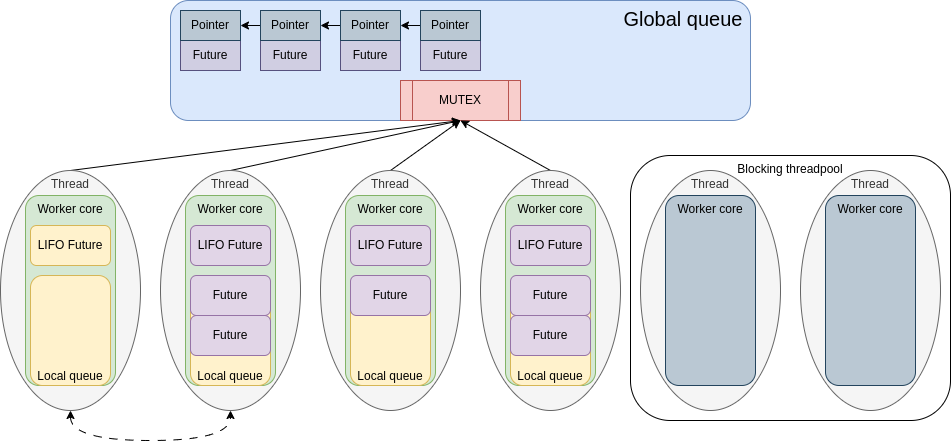
\includegraphics[scale=0.55]{pictures/tokio.arch.png}}
    \end{center}

    \caption{Упрощенное представление многопоточного рантайма}
    \label{fig:before}
\end{figure}

Блокирующие потоки ожидают определенный период, 10 секунд если не специфицировано иначе, поступления задач после чего прекращают свое исполнение.

\verb|Воркер|, так называется сущность ассоциированная с каждым из оставшихся \verb|worker_threads| потоков по средством размещения в локальной для этих поток переменной так называемого \verb|ядра воркера| --- структуры, необходимой для исполнения асинхронных задач, включающей \verb|локальную очередь|, хендлер \verb|глобальной очереди| и тому подобное.

\verb|Локальная очередь| воркера выступает в качестве кэша его задач, имеет фиксированный размер и предполагает добавление задач исключительно из потока владельца. Однако, изъятие из нее может быть осуществленно потоками других воркеров при нехватке оным собственных задач --- процесс называемый стилингом. Все это: фиксированный размер и производитель в единственном количестве позволяет ей иметь lock free алгоритм взаимодействия. В случае переполнения часть задач перемещается воркером в глобальную очередь.

\verb|Глобальная очередь| или \verb|inject queue| представляет собой коллекцию задач ожидающих исполнения. Наполняется она при спавнинге задачи вне контекста воркера или при переполеннии локальной очереди воркеров. Реализована с помощью интрузивного связного списка, защищенного мьютексом.

Исполнить асинхронное замыкание пользователь может несколькими способами:

\begin{itemize}
    \item \verb|block_on| --- метод инстанса рантайма позволяющий заблокировать поток приложения на исполнении определенного асинхронной задачи
    \item \verb|tokio::spawn| --- функция позволяющая поместить асинхронное замыкание в одну из очередей рантайма. Вызвов ее должен быть совершен в его контексте --- в одном из потоков, управляемых рантаймом, в методе \verb|block_on| или промежутке жизни объекта \verb|EnterGuard|. От места вызова будет зависеть, в какую очередь будет помещена задача: в случае потока воркер --- в локальную очередь, иначе --- глобальную
\end{itemize}

% TODO
\subsubsection{Выбор задачи}

Логика поиска воркером задачи для исполнения отражена на листинге \ref{listing:next_task}.

\begin{listing}
    \begin{minted}{rust}
fn next_task(&mut self) -> Option<Notified> {
    if self.tick % self.global_queue_interval == 0 {
        return next_remote_task()
                .or_else(|| self.next_local_task())
    }
    if Some(task) = self.next_local_task()  {
        return Some(task);
    }
    if inject().is_empty() {
        return None;
    }
    let (head, tail) = inject().pop_n(self.can_take());
    self.run_queue.push_back(tail);
    return head
}
    \end{minted}

    \caption{Логика выбора задачи}
    \label{listing:next_task}
\end{listing}

И осуществляется в следующем порядке: раз в определенное, конфигурируемое рантаймом, число тиков --- мера времени воркера, он пытается взять задачу из глобальной очереди, иначе --- из локальной, в остальное время проверяется локальная, после глобальная очереди.

\subsection{Цикл работы воркера}

Алгоритм рабочего цикла воркера отражен на листинге \ref{listing:worker:run}.

\begin{listing}
    \begin{minted}{rust}
fn run() {
    while !is_shutdown() {
        core.tick();
        if let Some(task) = core.next_task() {
            self.run_task(task, core);
            continue;
        }
        if let Some(task) = core.steal_work() {
            self.run_task(task, core);
            continue;
        }
        self.park(core)
    }
}
    \end{minted}

    \caption{Логика выбора следующей задачи}
    \label{listing:worker:run}
\end{listing}

А именно, воркер отсчиты тик, затем пытается взять найти задачу, после чего пытается украсть задачи у других воркеров. В случае неудачи он паркует поток.

\subsection{Метрики}

Метрики собираемые рантаймом предполагается использовать в двух направлениях:

\begin{itemize}
    \item Семплирование --- наблюдения поведения внутренних структур рантайма в определенный моменты исполнения задач
    \item Тотальная оценка --- анализ количеств тех или иных операций произведенных за весь период исполнения
\end{itemize}

К первому типу можно отнести глубину глобальной или локальных очередей в определенный момент времени. К последнему --- количество переполнений локальных очередей за все время исполнения. Стоит отметить, что количество переполнений без сомнений имеет смысл фиксировать и во время исполнения определенных сценариев, однако, семплинг не точен и с легкостью может упустить стремительно меняющиеся значения. Тогда как тотальная сумма не позволяет упускать отдельные опреции.

\verb|tokio-metrics| --- проект, предоставющий интерфейс для семплирования метрик рантайма. Далее будет представлен полный перечень метрик доступных из \verb|tokio-metrics|. Метрики будут разбиты на группы по аналогии для уменьшения повторений.

Группа предполагает перечисление в следующем порядке: значение представленное в tokio-metrics как общее значение для всех воркеров, минимум и максимум среди воркеров, оданко, для краткости в тексте будут обзоначены только именования суммарных.

\begin{itemize}
    \item \verb|total_park_count| --- количество парковок потоков воркеров
    \item \verb|mean_poll_duration| --- это значение представляет собой экспоненциально взвешенную скользящую среднюю продолжительности опросов задач
    \item \verb|total_noop_count| --- сколько раз поток воркера был распаркован, но не совершил никакой работы перед парковкой
    \item \verb|total_steal_count| --- количество задач, которые воркеры похитили, перместив их в свою локальную очередь
    \item \verb|total_steal_operations| --- количесво раз воркеры успешно похител задачи
    \item \verb|total_local_schedule_count| --- количество задач отправленных на исполенние из контектса воркера, что должна попасть в одну из локальных очередей
    \item \verb|total_overflow_count| --- сколько раз воркеры переполнили свои локальные очереди
    \item \verb|total_polls_count| --- количество опросов задач среди
    \item \verb|total_busy_duration| --- количество времени исполения задач
    \item \verb|total_local_queue_depth| --- количество задач помещенных в локальные очереди
\end{itemize}

И остальные:

\begin{itemize}
    \item \verb|workers_count| --- количество воркеров исполняющих задачи. Значение специфицируется при инстанциации рантайма

    \item \verb|poll_time_histogram| --- гистограмма опросов задач, сгруппированная по времени исполнения опросов

    \item \verb|num_remote_schedules| --- количество задач, отправленных на исполнение из вне. То есть количество задачи заспавненных вне контекста воркера, задач, попавших в глобальную очередь

    \item \verb|global_queue_depth| --- количество задач, помещенных в глобальную очередь
\end{itemize}

Для решения поставленных задач были выделены метрики, отражающие взаимодействие воркеров с очередями. То есть, метрики, демонстрирущие глубину глобальной очереди (\verb|global_queue_depth|), локальных очередей (\verb|total_local_queue_depth|), количество переполнений (\verb|total_overflow_count|), количество похищенных задач (\verb|total_steal_count|), количество удаленных спавнов (\verb|num_remote_schedules|).

\subsection{Бенчмаркинг}

Для измерений времени исполнения и пропускной способности была использована библиотека \verb|criterion|\footnote{\href{https://github.com/bheisler/criterion.rs}{Репозиторий} проекта criterion}. Так как она популярна, имеет обширную документацию, использовуется в \verb|tokio|.

\subsection{Изменения шедулера языка Go}

Как было отмечено ранее, алгоритмы шедулинга в tokio были созданы с оглядкой на реализацию рантайма языка Go. В свою очередь шедулинг корутин в Kotlin был сделать по мотивам tokio. С тех пор, никаких изменений рантайм Go не претерпел, точно так же, как рантайм языка Kotlin. Таким образом, все рантаймы предопологают наличия локальных очередей у воркеров и одной глобальной очереди с взаимноисключающим владением.


% % !TeX spellcheck = ru_RU
% !TEX root = vkr.tex

\section{Метрики}

% Метрики собираемые рантаймом предполагается использовать в двух направлениях:

% \begin{itemize}
%     \item Семплирование --- наблюдения поведения внутренних структур рантайма в определенный моменты исполнения задач
%     \item Тотальная оценка --- анализ количеств тех или иных операций произведенных за весь период исполнения
% \end{itemize}

% К первому типу можно отнести глубину глобальной или локальных очередей в определенный момент времени. К последнему --- количество переполнений локальных очередей за все время исполнения. Стоит отметить, что количество переполнений без сомнений имеет смысл фиксировать и во время исполнения, однако, семплирование с легкостью может упустить стремительно меняющиеся значения. Тогда как тотальная сумма не позволяет упускать отдельные операции.

% \subsection{Семплирование}

% \verb|tokio-metrics|\footnote{\href{https://github.com/tokio-rs/tokio-metrics}{Репозиторий} проекта tokio-metrics (Дата обращения: 4.1.2025)} --- проект, предоставляющий интерфейс для семплирования метрик рантайма и отдельных задач. Далее будет представлен полный перечень метрик доступных из \verb|tokio-metrics| для рантайма, так как применение их для отдельных задач найдено не было. Метрики будут разбиты на группы по аналогии для уменьшения повторений.

% Группа предполагает перечисление в следующем порядке: значение представленное в \verb|tokio-metrics| как общее значение для всех воркеров, минимум и максимум среди воркеров, однако, для краткости в списке будет обозначено только первое.

% \begin{itemize}
%     \item \verb|total_park_count| --- количество парковок потоков воркеров
%     \item \verb|mean_poll_duration| --- экспоненциально взвешенная скользящая средняя продолжительность опросов задач
%     \item \verb|total_noop_count| --- сколько раз воркер бездействовал между парковками
%     \item \verb|total_steal_count| --- количество похищенных задач воркерами
%     \item \verb|total_steal_operations| --- сколько раз воркеры похитили задачи
%     \item \verb|total_local_schedule_count| --- количество задач отправленных на исполнение из контекста воркера
%     \item \verb|total_overflow_count| --- сколько раз воркеры переполнили свои локальные очереди
%     \item \verb|total_polls_count| `--- количество опросов задач
%     \item \verb|total_busy_duration| --- суммарное время исполнения задач
%     \item \verb|total_local_queue_depth| --- количество задач помещенных в локальные очереди
% \end{itemize}

% И остальные:

% \begin{itemize}
%     \item \verb|workers_count| --- количество воркеров

%     \item \verb|poll_time_histogram| --- гистограмма времени опросов задач

%     \item \verb|num_remote_schedules| --- количество задач, отправленных на исполнение из вне

%     \item \verb|global_queue_depth| --- количество задач находящихся в глобальной очереди
% \end{itemize}


% \subsection{Тотальные метрики}

\verb|tokio| предоставляет интерфейс для экстракции метрик из инстанса рантайма. Соответственно, для получения необходимо лишь опрашивать предварительно подверженный необходимым условиям инстанс.

Общие метрики для рантайма:

\begin{itemize}
    \item \verb|num_workers| --- количество воркеров
    \item \verb|num_alive_tasks| --- количеств исполняемых рантаймом задач
    \item \verb|global_queue_depth| --- количество задач в глобальной очереди
    \item \verb|num_blocking_threads| --- количество блокирующих потоков
    \item \verb|num_idle_blocking_threads| --- количество простаивающих блокирующих потоков
    \item \verb|spawned_tasks_count| --- количество созданных задач
    \item \verb|remote_schedule_count| --- количество задачи созданных вне контекста воркера
    \item \verb|budget_forced_yield_count| --- количество задач вытесненных рантаймом с исполнения
    \item \verb|blocking_queue_depth| --- количество задач в очереди блокирующего пулла
\end{itemize}

Метрики вычисляемые отдельно для каждого воркера:

\begin{itemize}
    \item \verb|worker_thread_id| --- получения внутреннего идентификатора воркера
    \item \verb|worker_park_count| --- количество парковок потока воркера
    \item \verb|worker_park_unpark_count| --- сумма парковок и распарковок
    \item \verb|worker_noop_count| --- количество бездействий между парковками
    \item \verb|worker_steal_count| --- количество похищенных задач
    \item \verb|worker_steal_operations| --- количество похищений
    \item \verb|worker_poll_count| --- количество опросов задач
    \item \verb|worker_total_busy_duration| --- время исполнения воркером задач
    \item \verb|worker_local_schedule_count| --- количество созданных в контексте воркера задач
    \item \verb|worker_overflow_count| --- количество переполнений локальной очереди
    \item \verb|worker_local_queue_depth| --- количество элементов в локальной очереди
    \item \verb|worker_mean_poll_time| --- экспоненциально взвешенная скользящая средняя продолжительность опросов задач
\end{itemize}

Метрики описывающие время опроса задач в виде гистограмм:

\begin{itemize}
    \item \verb|poll_count_histogram_enabled| --- включен ли сбор гистограмм количества опросов

    \item \verb|poll_time_histogram_num_buckets| --- количество значений гистограммы

    \item \verb|poll_time_histogram_bucket_range| --- значения гистограммы
\end{itemize}

Так как метрики будут получены после исполнения, ценность имеют лишь показатели накапливающие значение на протяжении сценария и сохраняющие его после. К таким можно отнести количество парковок потока воркера (\verb|worker_park_count|) или временные гистограммы опроса задач (\verb|poll_time_histogram_bucket_range|). Метрики диагностирующие состояние структур в определенный момент времени, например, глубину глобальной или локальных очередей, после исполнения бенчмарка имеют не большое значение, ибо должны быть равны нулю. Однако, именно это ``должны быть'' можно и нужно подвергать дополнительной проверке в качестве пред и постусловий.

\subsection{Выделенные метрики}

Для решения поставленных задач были выделены метрики, отражающие взаимодействие воркеров с очередями. То есть метрики, демонстрирующие глубину глобальной очереди (\verb|global_queue_depth|), локальных очередей (\verb|total_local_queue_depth|), количество переполнений (\verb|total_overflow_count|), количество похищений (\verb|total_steal_operations|), количество удаленных спавнов (\verb|num_remote_schedules|).

Для самопроверки были выделены временные гистограммы исполнения задач (\verb|poll_time_histogram_bucket_range|), количества воркеров (\verb|num_workers|), количество исполняемых задач (\verb|num_alive_tasks|) и тому подобные.

\subsection{tokio-metrics}

\verb|tokio-metrics|\footnote{\href{https://github.com/tokio-rs/tokio-metrics}{Репозиторий} проекта tokio-metrics (Дата обращения: 4.1.2025)} --- проект, предоставляющий интерфейс для семплирования метрик рантайма и отдельных задач. Перечень метрик коего упускается, так как пользы семплирование в ходе этой работы не принесло.

% !TeX spellcheck = ru_RU
% !TEX root = vkr.tex

\section{Система бенчмарков}

Бенчмарки в репозитории проекта \verb|tokio| не пригодны для анализа производительности в рамках данной работы, так как используют методы синхронизации имеющие не тривиальный эффект на результатах экспериментов:

\begin{itemize}
    \item Атомарное чтение и запись из множества исполняемых разными потоками задач скорее позволяет измерять производительность системы памяти физической машины, нежели взаимодействия структур рантайма~\cite{atomicOnModerHardware}.
    \item Ожидание исполнения в методе \verb|block_on| \verb|tokio| рантайма чревато неточным измерением из-за текущей реализации\footnote{\href{https://github.com/bheisler/criterion.rs/issues/819}{Проблема} измерения производительности асинхронных функций (Дата обращения: 4.1.2025)}.
\end{itemize}

Поэтому в качестве системы бенчмарков был создан проект \verb|tokiobench|\footnote{\href{https://github.com/IgorErin/tokiobench}{Репозиторий} проект tokiobench (Дата обращения: 4.1.2025)}, где предполагалось реализовать сценарии использования проекта \verb|tokio| в \verb|TATLIN.BACKUP|. При общении с командой \verb|TATLIN.BACKUP| был выделен основной сценарий, представленный на рисунке~\ref{fig:scenario}:

\begin{figure}[H]
    \begin{center}
        \makebox[\textwidth]{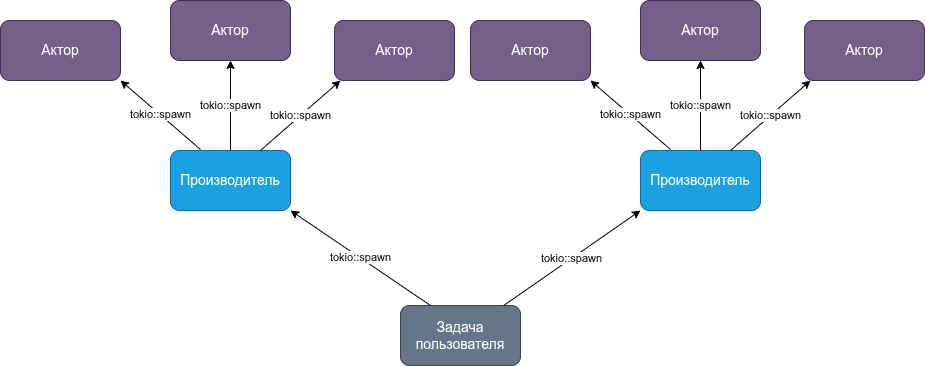
\includegraphics[scale=0.55]{pictures/scenario.drawio.png}}
    \end{center}

    \caption{Основной сценарий использования tokio в TATLIN.BACKUP.}
    \label{fig:scenario}
\end{figure}

\begin{itemize}
    \item Актор --- замыкания, в цикле ожидающие асинхронные события.
    \item Производитель --- замыкания, отправляющее на исполнение множество замыканий акторов.
\end{itemize}

Необходимо было исследовать производительность такого сценария при следующих параметрах:

\begin{itemize}
    \item Тысяча замыканий акторов.
    \item Тысяча итераций исполнения акторов.
    \item Сто замыканий производителей.
\end{itemize}

\subsection{Реализация бенчмарков}

Методы реализации бенчмарков из \verb|tokio| были улучшены:

\begin{itemize}
    \item Атомарные переменная была заменена иерархией заранее аллоцированных переиспользуемых от итерации к итерации буферами, коллекционирующими структры типа \verb|JoinHandle|.
    \item Ожидание структур типа \verb|JoinHandle| перенесено в отдельную задачу, которая сообщает о завершении обработки с помощью блокирующего канала.
\end{itemize}

Накладные расходы, вызванные использованием блокирующего канала были приняты во внимание, поэтому, исключительно для проверки, была создана реализация использующая спинлок: фиксирующий исполнение и сигнализирующий поток пишет значение в атомарную переменную --- поток бенчмарка ожидает этого в цикле.

Для эмуляции операций ввода вывода был использован метод \verb|yield_now()|: каждый актор тысячу раз выполняет \verb|yield_now()|, что заставляет исполнителя сохранять структуру типа \verb|Waker| в локальной коллекции, для последующего вызова метода \verb|wake()|. Вызов метода \verb|wake()| приводит к переполнению локальной очереди исполнителя, вынуждая последнего перемещать задачи из локальной очереди в глобальную. После исполнения задач из локальных очередей исполнители начинают обращаться к глобальной очереди, затем похищают задачи друг у друга. Такая реализация заставляет исполнителей часто взаимодействовать, что способствует оценке накладных расходов этого взаимодействия и вызванных им синхронизаций.

% !TeX spellcheck = ru_RU
% !TEX root = vkr.tex

\section{Исследование производительности tokio}

Целями данной главы является изучение изменения производительности при разделении константного количества исполнителей между различным количеством инстансов асинхронных рантаймов: если синхронизации исполнителей накладывают ограничение на производительность системы, использующей один асинхронный рантайм, использование нескольких асинхронных рантаймов с меньшим количеством исполнителей должно продемонстрировать большую пропускную способность.

\subsection{Условия экспериментов}\label{experiment_environment}

Для измерения производительности была использована библиотека \verb|criterion|\footnote{\href{https://github.com/bheisler/criterion.rs}{Репозиторий} проекта criterion (Дата обращения: 25.5.2025).}. Так как она популярна, имеет обширную документацию и используется в \verb|tokio|.

Здесь и далее эксперименты производились при следующих условиях:

\begin{itemize}
    \item Исследования проводились на системе YADRO VEGMAN Rx20 G2\footnote{\href{https://yadro.com/ru/vegman/rx20g2/specs}{Описание} системы YADRO VEGMAN Rx20 G2 (Дата обращения: 25.5.2025).}.
    \item Бенчмарк был запущен со значением \verb|nice| равным минус двадцати.
    \item Исполнение было рекомендовано на одной NUMA единице с помощью \verb|taskset|.
\end{itemize}

Машина для измерения производительности была предоставлена командой \verb|TATLIN.BACKUP| и использовалась удаленно, в связи с чем на ней было невозможно отключение сети.

Библиотека \verb|criterion| имела следующую конфигурацию:

\begin{itemize}
    \item Пять секунд прогрева.
    \item Сорок семплов для каждого измерения.
    \item Линеаризация в качестве способа семплирования.
\end{itemize}

\subsection{Ход исследования}

Для проверки гипотезы об ограничении производительности ресурсами одного рантайма, были произведены измерения пропускной способности системы, состоящей из нескольких рантаймов, приведенные на графике \ref{fig:tatlin:multi_rt:eval}. Каждое измерение использовало одинаковое количество потоков исполнителей и задач производителей, равномерно разделенных между рантаймами.

\begin{figure}[H]
    \begin{center}
        \makebox[\textwidth]{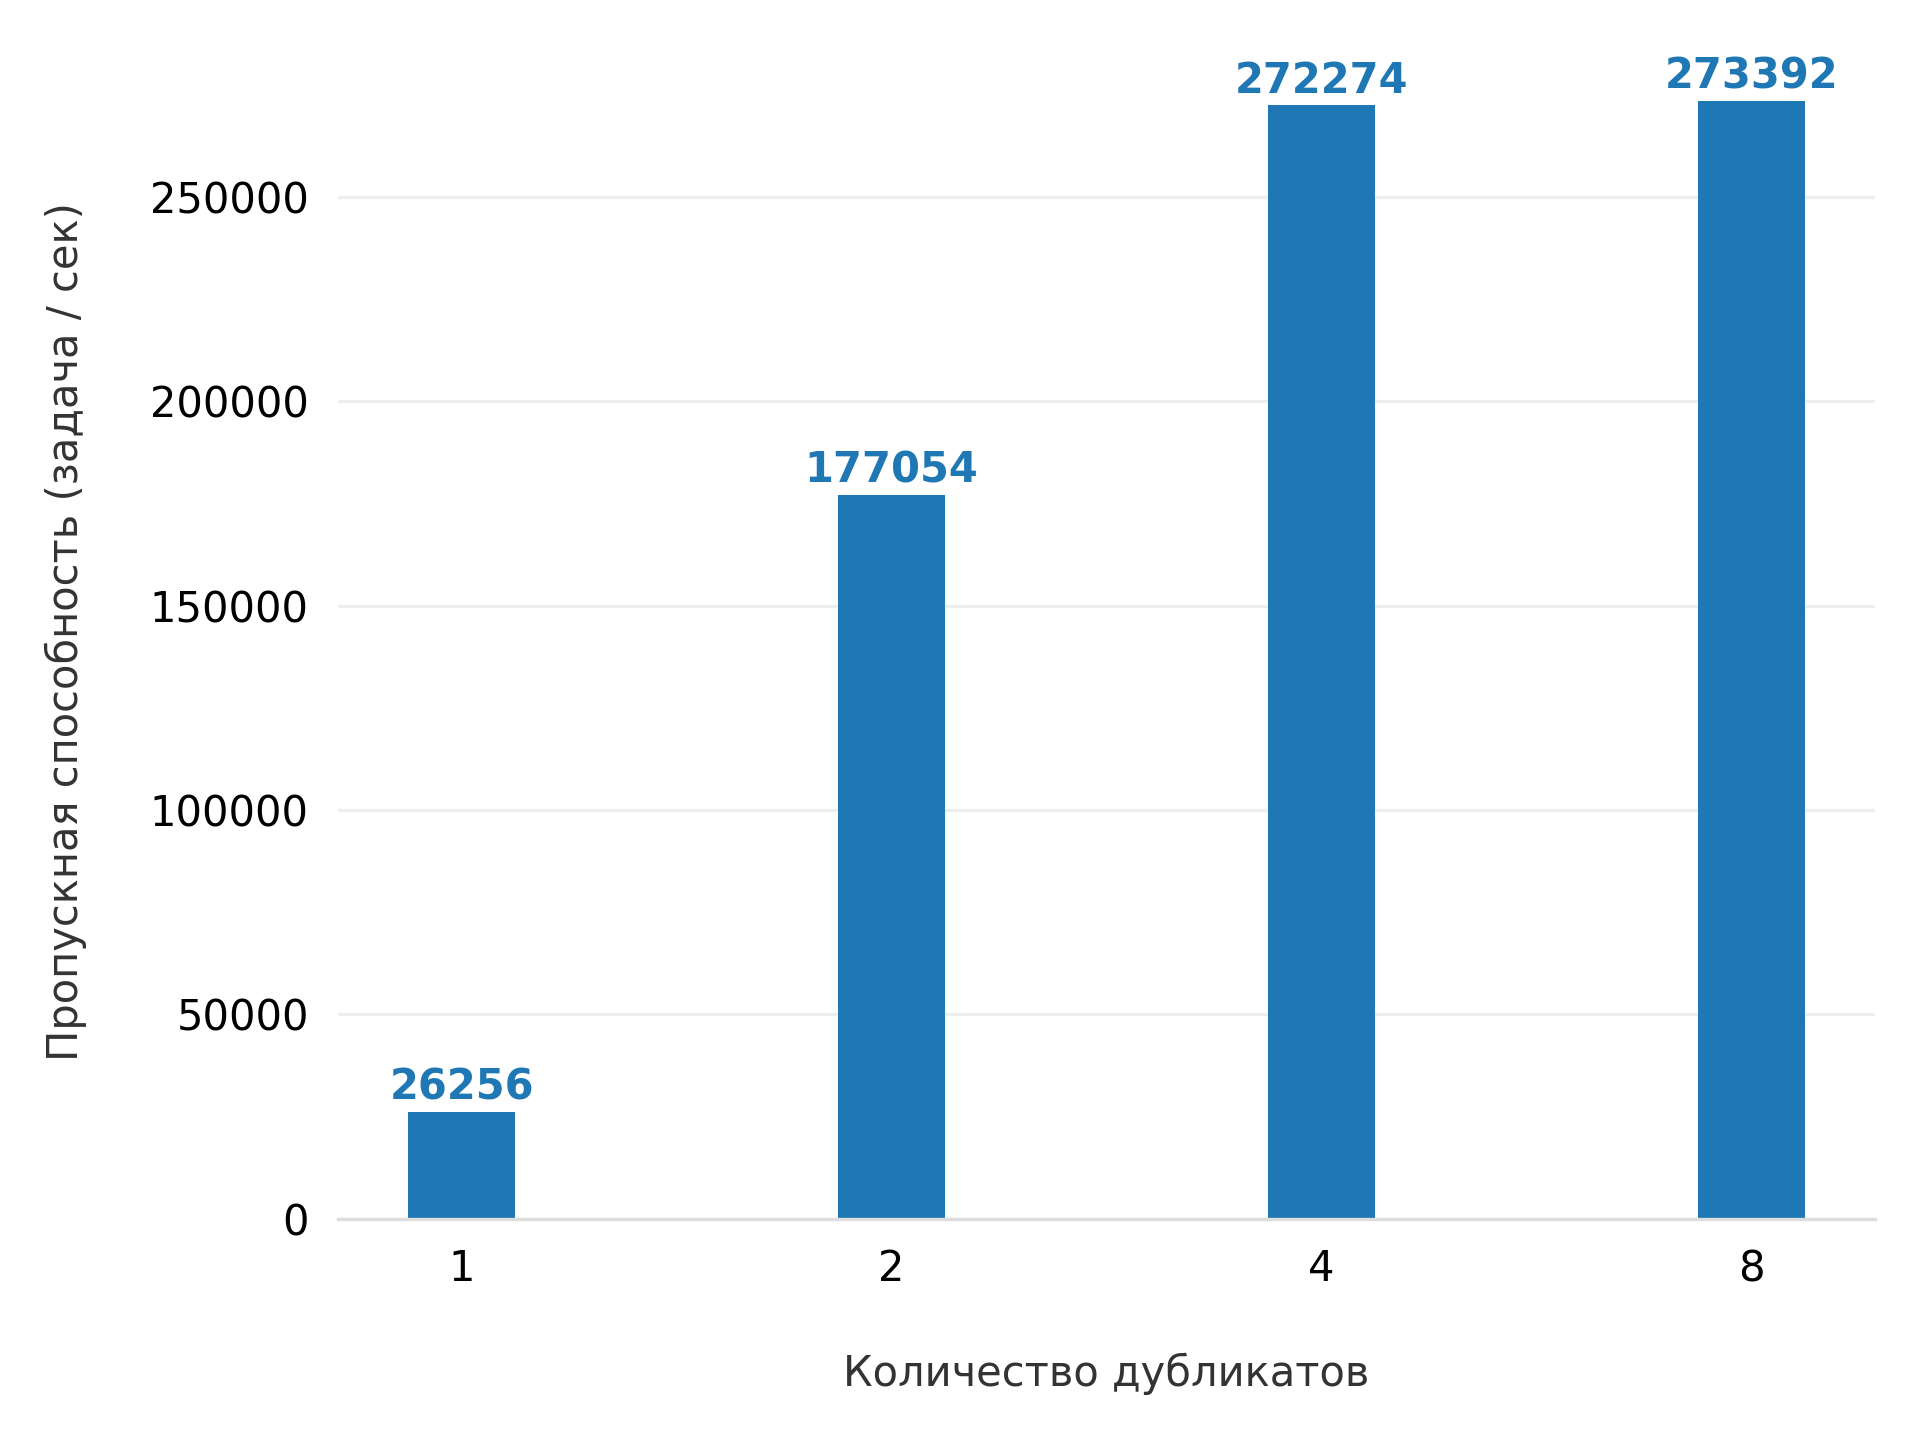
\includegraphics[scale=0.90]{pictures/rt_nsapwner128_nspawn1000.png}}
    \end{center}

    \caption{Производительность системы при использовании нескольких рантаймов.}
    \label{fig:tatlin:multi_rt:eval}
\end{figure}

Из изображения заметным становится увеличение производительности при увеличении количества рантаймов, то есть разделение задач между меньшими изолированными группами исполнителей позволяет увеличить пропускную способность.

\subsection{Вывод}

При изоляции меньших групп исполнителей с отдельными глобальными очередями в рамках отдельных инстансов рантаймов наблюдается увеличение пропускной способности. Это может происходить из-за уменьшения количества синхронизаций между исполнителями.

\begin{itemize}
    \item Меньшая борьба за глобальную очередь, за счет деления исполнителей между несколькими очередями.
    \item Меньшее количество исполнителей пытаются украсть задачи у соседей из-за изоляции исполнителей в различных инстансах рантайма.
\end{itemize}

Таким образом, шардирование рантайма позволяет увеличить пропускную способность системы.

% !TeX spellcheck = ru_RU
% !TEX root = vkr.tex

\section{Проектирование решения}

После полученных результатов команда \verb|TATLIN.BACKUP| провела эксперименты, где так же стало очевидно преимущество использования нескольких рантаймов с точки зрения пропускной способности.

Однако, неясным осталась надежность такой системы: разработчики tokio не дают никаких гарантий относительно взаимодействия такой системы, а наоборот утверждают, что при некотором обращении с такой конструкцией могут быть наблюдаемы падения производительности или достижимо неопределенное поведение. \verb|TATLIN.BACKUP| позиционирует себя как высоконадежное производительное решение, а потому использовать в нем конструкцию без гарантий не возможно.

\subsection{Шардирование глобальной очереди}

Если дублировать весь рантайм нельзя, вероятно, уменьшить ограничение накладываемое глобальной очередью получится при использовании нескольких глобальных очередей в одном рантайме, как представленно на изображении~\ref{fig:tokio:duplicated_arch}.

\begin{figure}[H]
    \begin{center}
        \makebox[\textwidth]{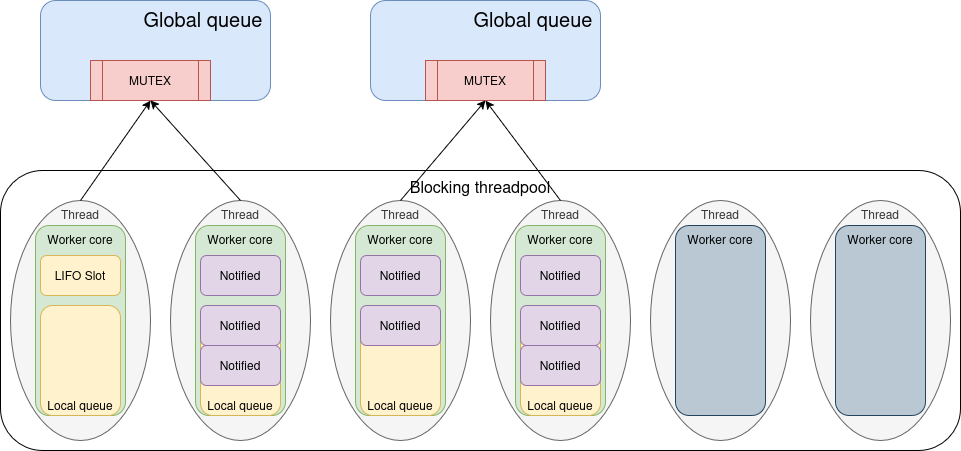
\includegraphics[scale=0.55]{pictures/tokio_duplicated.drawio.png}}
    \end{center}

    \caption{Упрощенное представление многопоточного рантайма}
    \label{fig:tokio:duplicated_arch}
\end{figure}
Здесь и далее под рабочей группой будет пониматься глобальная очередь с фиксированным количеством воркеров.

Это было реализовано с следующими измененями в интерефейсе tokio:

\begin{itemize}

\item При создании рантайма пользователь специфицирует количество групп (\verb|worker_groups|) и количество количество воркеров в каждой группе (\verb|worker_threads|). В результате рантайм инстанциируется с \verb|worker_threads| * \verb|worker_groups| системными потоками для исполнения асинхронных замыканий.
\item Для отправки замыкания исполняться в определенную рабочую группу добавлен метод \verb|tokio::spawn_into|.
\end{itemize}


Рабочая группа выбирается с помощью локального для потока рандома~\cite{xorshiftRNG} в следующих случаях:

\begin{itemize}
    \item Создании задачи с в процессе аллокации замыкания с методом \verb|tokio::spawn|
    \item Отправки \verb|Notified| в планировщик tokio в следствии готовности системных ресурсов
\end{itemize}

Каждая группа изолирована от остальных, то есть воркеры не могут похищать задачи из глобальных очередей или локальных очередей воркеров из других групп. Это вынуждает их быть запаркованными при нехватке задач в собственной группе, что позволяет:

\begin{itemize}
    \item Избежать конфликтов между воркерами из различных групп.
    \item Экономить системные ресурсы.
\end{itemize}

При появлении задач будет разбужено соответствующее количество воркеров в соответствующей группе.

\subsection{Индентификатор задач}

При создании задачи для нее генерируется индентификатор на одной статической ячейке памяти, переменной разделяемой между всеми попытками создать задачу в рамках процесса. То есть при создании каждой задачи, пусть даже в различных потоках, устанавливается глобальный порядок на одной ячейке памяти для поддержания уникальности индентификаторов.

Этого можно избежать если, индентификатор будет состоять из двух частей как представлено на листинге~\ref{listing:id:composite} --- в таком случае можно инстанциировать несколько производителей различных индентификаторов.

\begin{listing}[H]
    \begin{minted}{rust}
struct Id {
    head: u64,
    tail: u64,
}
    \end{minted}

    \caption{Асинхронное замыкание}
    \label{listing:id:composite}
\end{listing}

А именно: на статической атомарной перменной будет производиться генерации первой части индентификатора задачи, так называемого индентификатора производителя индентификаторов задач, представленного на листинге~\ref{listing:id:provider}

\begin{listing}[H]
    \begin{minted}{rust}
struct IdProvider {
    head: u64,
    tail_counter: AtomicU64,
}
    \end{minted}

    \caption{Асинхронное замыкание}
    \label{listing:id:provider}
\end{listing}

каждый из которых будет иметь собственную атомарную ячейку памяти для генерации индентификаторов задач.

При создании задачи ее необходимо зарегистрировать в \verb|OwnedTasks|, путем выбора шарда и помещению в него указателя \verb|Task|. Выбор шарда ранее происходил с помощью индентификатора задачи, то есть использование шардов происходило последовательно. Однако, при использовании составного индентификатора повышается возможность конфликта при выборе шарда, что значительно снижает производительность. Поэтому в данный момент применение составному индентификатору не найдено.


% !TeX spellcheck = ru_RU
% !TEX root = vkr.tex

\section{Заключение}

В ходе работы были выполнены следующие задачи:

\begin{itemize}
    \item Получено первое описание реализации tokio с точки зрения асинхронного интерфейса языка \verb|Rust|. В результате обзора выявлены две возможные уязвимости с точки зрения производительности: взаимодействие исполнителей и реализация глобальной очереди. Первая уязвимость была устранена в результате текущей работы путем шардирования планировщика многопоточного рантайма. Изменение многопоточного рантайма с точки зрения алгоритмов глобальной очереди рассмотрены в ВКР Матвея Калашникова: ``Оптимизация системы управления очередью задач в библиотеке Tokio для асинхронного рантайма''.
    \item Создан проект, содержащий бенчмарки, позволяющий автоматически собирать метрики и визуализировать результаты\footnote{\href{https://github.com/IgorErin/tokiobench}{Репозиторий} проект tokiobench (Дата обращения: 25.5.2025)}.
    \item Произведен эксперимент, основанный на ключевом сценарии использования \verb|tokio| в \verb|TATLIN.BACKUP|. Обнаружена возможность увеличить пропускную способность \verb|TATLIN.BACKUP|, что может свидетельствовать о существовании ограничения, накладываемого глобальной очередью. Однако, такой подход остается небезопасным.
    \item Предложена и реализована безопасная модификация рантайма, позволяющая использовать несколько глобальных очередей в одном инстансе рантайма\footnote{\href{https://github.com/IgorErin/tokio/pull/3}{Реализация} шардирования многопоточного рантайма. Имя пользователя: IgorErin (Дата обращения: 25.5.2025)}.
    \item Проведены эксперименты на целевом сценарии \verb|TATLIN.BACKUP|, показавшие увеличение производительности предложенного решения.
\end{itemize}

Языковые асинхронные интерфейсы трудны в создании вследствие необходимости наличия высокопроизводительной реализации для различных сред: будь то приложения для встроенных систем~\cite{CPPCoroutinesOnMicrocontrollers, AsyncIOT} или пользовательские программные продукты, способные эффективно исполняться на различных архитектурах и операционных системах~\cite{CPPCoroutinesDesignAndImpl}.

Известно множество исследований, направленных на изучение создания и оптимизации пуллов для исполнения вычислительных задач~\cite{ThreadPoolSize, PerfDeviationsInThreadPools, SyncInThreadPools, ProduserConsumerThreadPool}. Однако автору не удалось найти академические работы, посвященные реализации языковым асинхронных рантаймов. Вероятно, это связано с относительно недавним их появлением в языках с повышенным контролем над ресурсами~\cite{CPPCoroutinesDesignAndImpl}.

Стоит отметить, что асинхронные движки таких популярных языков, как Go, Kotlin, tokio в экосистеме языка Rust представляют собой вариации дизайна, предложенного Дмитрием Вьюковым для языка Go~\cite{GoScheduler, GoSchedulerImpropvements}. Данная работа показывает, что незначительные изменения в этом популярном подходе могут увеличить пропускную способность отдельных бенчмарков на порядок, что может свидетельствовать о необходимости дальнейших исследований использования современных асинхронных интерфейсов~\cite{ModernStorageAPI} и подходов к многопоточности~\cite{ThreadPerCore}.

% % !TeX spellcheck = ru_RU
% !TEX root = vkr.tex

\section{Terms}

wait freedom: each thread moves forward regardless of external factors like contention from other threads, other thread blocking
lock freedom: system as a whole moves forward regardless of anything
obstruction-freedom: thread makes forward progress only if it does not encounter contention from other threads
    - blocked/interrupted/terminated threads can not prevent progress of other threads
    - obstruction-free algorithms can be faster than lockfree algorithms
termination-safety: terminated thread does not prevent system-wide forward progress
blocking: allow a slow or delayed process to prevent faster processes from completing operations on the shared data structure indefinitely
non blocking: guarantee that if there are one or more active processes trying to perform operations on a shared data structure, some operation will complete within a finite number of time steps

linearizable: An implementation of a data structure is linearizable if it can always
give an external observer, observing only the abstract data structure opera-
tions, the illusion that each of these operations takes effect instantaneously
at some point between its invocation and its response


\setmonofont{CMU Typewriter Text}
\bibliographystyle{ugost2008ls}
\bibliography{vkr}

\end{document}
